Постановка представляет тест как стохастический ряд вида $\{x\}_{t=0}$ каждый элемент, которого является случайной бернуллевской величиной с параметром $s$. 
Для ввода управляющей переменной задается сложность задачи $d$, параметризующий в совокупности с функцией отклика учащегося $f$, переменную $s_t = f(d)$.

 Таким образом, задача алгоритма предложить функцию $f(d_{t+1}^t,{x}_{i=0}^t)$, обеспечивающую оптимальную сходимость $\lim_{t \rightarrow \infty} \rho(s(d_t),s^*) =1$ согласно условиям:
 \begin{itemize}
    \item метрика $\rho(x,x') = (x-x')^2$ евклидова
    \item предполагается наличие банка $W$, возвращающего задачу произвольной сложности $d$
    \item функция отклика $f(d_t)$ ограничена числом $M$ и монотонно убывает
\end{itemize}

Алгоритм, отвечающий заданным требования  был предложен в работе \cite{yazidi2020balanced}. Авторы предложили правило обновления сложности:

\begin{equation}
    d_{t+1} = \Pi(d_t+\lambda (x(t) -s^*)),
    \label{yazidi}
\end{equation}
где функция $\Pi$ является ограничивающим оператором вида
\begin{equation}
    \Pi_H(d) = \left\{
        \begin{array}{ll}
            d,\ \text{прт}\ 1<d<0 \\
            1,\ d\ge 1\\
            0, \text{при} \ d \le 0\\
        \end{array}
    \right.
\end{equation}

Алгоритм по форме соответствует алгоритму Роббинса-Монро\cite{robbins1951stochastic}, известному в теории стохастической аппроксимации. 
Отметим, что поскольку коэффициент $\lambda$ является постоянной, то сходимость по алгоритму Роббинса-Монро не гарантируется.


\begin{equation}
    x_{n+1} = x_{n} - a_n(x -b_n).
\end{equation}
Схема доказательства \begin{enumerate}
    \item используем модифицированный алгоритм Роббинса-Монро, используя 
    \item зададим связь между функцией отклика $s(d)$ и параметрами $a_n$ и $b_N$ через условия несмещенности оценки $E(x_n)$ и
минимизации дисперсии $\mathbf{D}(x_n) \rightarrow min$  \cite{hu1997strong} \cite{hu1998sequential}
    \item определим явное выражение $a_n$ и $b_n$ для априорного представления о функции отклика в виде параметрической модели Эло $s(d,\alpha,\beta) = 1 - \frac{1}{1+\exp\left(-\beta \cdot(\mathbf{d} -\alpha)\right)}$
\end{enumerate}

\begin{figure}[h!]
    \centering
    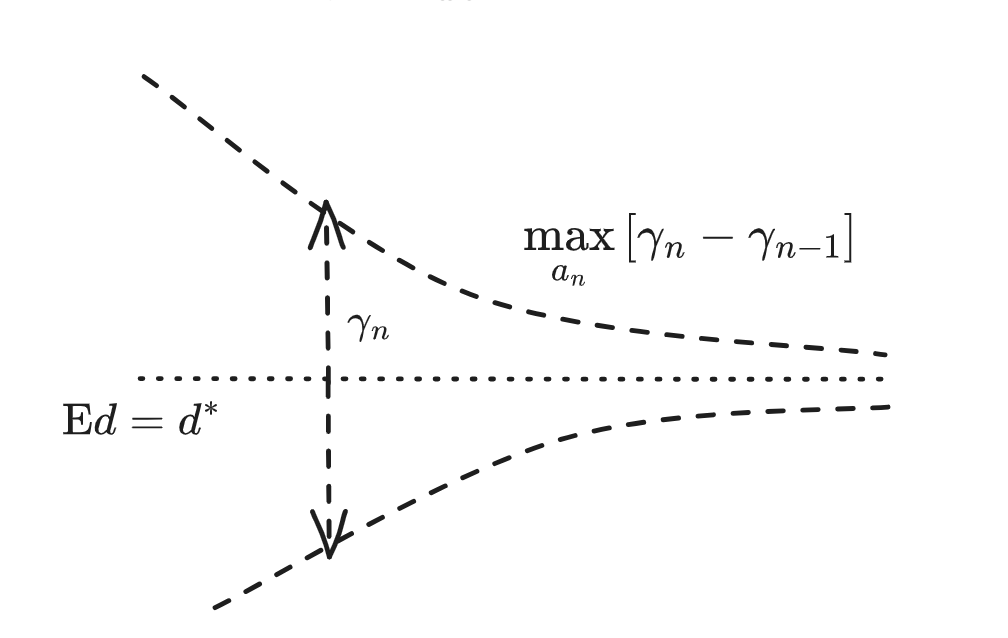
\includegraphics[width=0.5\textwidth]{assets/work/rating/dispersion_reduction.png}
    \caption{Использование несмещенной оценки с постепенной редукцией дисперсии}
    \label{principal_scheme}
\end{figure}

\textit{\textbf{Теорема.}Адаптированный алгоритм Роббинса-Монро для случая наблюдений, имеющих бернуллевское распределение.} \label{algo} 
При условии $\forall n \rightarrow x_n \sim \text{Bern}(s(d_n))$ выполняются следующие утверждения. \begin{enumerate}
    \item Оптимальная сходимость достигается при $a_n = \frac{\mathbb{E}[d_n s(d_n)]}{\mathbb{E}s(d_n)(1 - \mathbb{E}s(d_n))}$ , $b_n =\mathbb{E} s(d_n)$
    \item Для функции отклика, представленной параметрической моделью Эло $s(d,\alpha,\beta) = 1 - \frac{1}{1+\exp\left(-\beta \cdot(d -\alpha)\right)}$
     и в предположении нормальности распределения $d \sim \mathcal{N}(\alpha,\sigma^2)$ получим аппроксимацию рядов $a_n$ и $b_n$, обеспечивающих оптимальную сходимость как\begin{itemize}
        \item $a_n = \frac{1}{b_n(1-b_n)} \frac{1}{4  \beta \sqrt{1+\frac{\pi\gamma_n^2}{8}}} \exp\left( \frac{- \pi (\alpha-d^*)^2}{16  \beta^2 ( 1+\frac{\pi\gamma_n^2}{8})}\right)$
        \item $b_n = \frac{1}{2} + \frac{1}{2} \text{erf}\left(\frac{\sqrt{\pi} (\alpha-d^*)}{4 \sqrt{1+\frac{\pi\gamma_n^2}{8}}} \right)$.
    \end{itemize} 
\end{enumerate}
\textit{Доказательство}
Сходимость метода приведена в аппендиксе работы \ref{ino}.
1) Используем рекуррентное представление для поиска оптимальных параметров $a_n,b_n$
\begin{equation}
    d_{n+1} = d_n -  a_n(x_n-b_n).
    \label{mod_scheme}
\end{equation}
Рассчитаем матожидание $\mathrm{E}_{d_n ~ p(d_n)}$ как:
\begin{equation}
    \mathrm{E} d_{n+1} = \mathrm{E} d_n -  a_n(\mathrm{E}x_n-b_n).
\end{equation}
Запишем условия $\mathrm{E} d_{n+1} = d^*$ c учетом $\mathrm{E} d_{n} = \dots \mathrm{E} d_{1}= d^*$:
\begin{equation}
    a_n (\mathrm{E} s(d_n) - b_n)  =0.
\end{equation}
Следовательно,
\begin{equation}
    \label{b_n}
    b_n = \mathrm{E} s(d_n).
\end{equation}
Коэффициент $a_n$ найдем из минимизации дисперсии $\mathbf{D} d_{n+1}$. Запишем $\mathbf{D}_{x_n \sim Bern(x | s(d_n))}$ для выражения \ref{mod_scheme}:
\begin{equation}
    \label{disp}
    \mathbf{D} d_{n+1} = \mathbf{D} d_n + a_n^2 \mathbf{D} (x_n-b_n)  - 2 a_n \mathrm{E}\left[(x_n-b_n)d_n\right].
\end{equation}
Поскольку $x_n \sim \text{Bern}(s(d_n))$,то
\begin{equation}
    \mathbf{D}(x_n-b_n) = \mathrm{E} s(d_n) \mathrm{E} (1-s(d_n))=  \mathrm{E} s(d_n)  (1-\mathrm{E}s(d_n)).
\end{equation}
С учетом $b_n = \mathrm{E} s_d$ и $\mathrm{E} d_n =d^*$:
\begin{equation}
    \mathrm{E}\left[(x_n-b_n)d_n\right] = \mathrm{E}\left[x_n d_n \right] - b_n  \mathrm{E} d_n = \mathrm{E} \left[s(d_n) d_n\right] - \mathrm{E} s(d) d^*.
\end{equation}
Тогда:
\begin{equation}
    \mathbf{D} d_{n+1} = \mathbf{D} d_n + a_n^2 \mathrm{E}s(d_n)\mathrm{E}(1-s(d_n)) - 2 a_n \mathrm{E}\left[ s(d_n) (d_n-d^*)\right].
\end{equation}
Из условия $\frac{\partial \mathbf{D}{d_{n+1}}}{\partial a_n} =0 $ получаем:
\begin{equation}
    \label{diff}
    a_n = \frac{\mathrm{E} \left[ (d_n-d^*) s(d_n)\right]}{\mathrm{E}s(d_n)(1 - \mathrm{E}s(d_n))}.
\end{equation}
Тогда связь между дисперсиями на каждом шаге запишется как:
\begin{equation}
    \mathbf{D} d_{n+1} = \mathbf{D} d_n - \frac{\left(\mathrm{E} \left[ (d_n-d^*) s(d_n)\right] \right)^2}{\mathrm{E}s(d_n)(1 - \mathrm{E}s(d_n))} 
\end{equation}
2) Определим оптимальные коэффициенты $a_n$ и $b_n$ для случая отклика согласно модели Эло: $s(d_n) = \sigma(d,\alpha,\beta) = 1 - \frac{1}{1+\exp(-\frac{(d_n-\alpha)}{\beta})}$. Исходя из предположения $d^*$:
\begin{equation}
    d^* = \alpha  - \beta \log\left(\frac{s^*}{1-s^*}\right).
\end{equation}
Согласно условию $d$ распределен нормально $\sim \mathcal{N}(\alpha_n,\gamma_n)$. $\alpha_n = d^*$, исходя из несмещенности оценки $d_n$. $\gamma_n$ рекуррентно связан с значениям предыдущих операций согласно \ref{diff}:
\begin{equation}
    \label{gamma_connection}
    \gamma_n = \gamma_{n-1} - \frac{\left(\mathrm{E} \left[ (d_n-d^*) s(d_n)\right] \right)^2}{\mathrm{E}s(d_n)(1 - \mathrm{E}s(d_n))}.
\end{equation}
Найдем $b_n$ из \ref{b_n}:
\begin{equation}
    b_n = \int_{-\infty}^{\infty} s(x) \mathcal{N}_{d^*,\gamma_n}(x) d x = \int_{-\infty}^{\infty} \sigma(x,\alpha,\beta) \mathcal{N}_{d^*,\gamma_n} d x.
\end{equation}
Для этого используем аппроксимацию логнормальныого интеграла через функцию ошибки $\text{erf}(x) = \int_{-\infty}^x \exp(-t^2)$:
\begin{equation}
     \sigma(x, \alpha, \beta) \approx \frac{1}{2} + \frac{1}{2} \text{erf}\left(\frac{(x-\alpha)\sqrt{\pi}}{4 \beta}\right).   
\end{equation}
Свертка  $\text{erf}(x)$ c плотностью вероятности гауссового распределения $\mathcal{N}(d^*,\gamma_n)$ является табличным интегралом \cite{ng1969table}:
\begin{equation}
    b_n \approx \int_{-\infty}^{\infty} \left[\frac{1}{2} + \frac{1}{2} \text{erf}\left(\frac{\sqrt{\pi}}{4\beta} (x-\alpha) \right) \right] \mathcal{N}_{d^*,\gamma_n}(x) dx = 
    \frac{1}{2} + \frac{1}{2} \text{erf}\left(\frac{\sqrt{\pi} (\alpha-d^*)}{4 \beta \sqrt{1+\frac{\pi\gamma_n^2}{8}}} \right).
\end{equation}
Найдем $a_n$ из \ref{diff}:
\begin{equation}
    \label{a_n}
    \begin{aligned}
          a_n &= \frac{1}{b_n(1-b_n)} \int_{-\infty}^{\infty} d (\sigma(x\alpha,\beta) -d^*) \mathcal{N}_{d^*,\tau}(x)  dx \\  
          &\approx  \int_{-\infty}^{\infty} x \left[\frac{1}{2} - d^* + \frac{1}{2} \text{erf}\left(\frac{(x-\alpha)\sqrt{\pi}}{4 \beta}\right)\right] \mathcal{N}_{d^*,\gamma_n}(x) dx \\
          &= \frac{d*}{2 \gamma_n^2} \text{erf}\left(\frac{\sqrt{\pi} (\alpha-d^*)}{4 \sqrt{1+\frac{\pi\gamma_n^2}{8}}} \right)  + \frac{1}{4 \gamma_n^2} \frac{1}{b_n(1-b_n)} \int_{-\infty}^{\infty} x \text{erf}\left(\frac{(x-\alpha)\sqrt{\pi}}{4 \beta}\right) \exp\left(\frac{(x-d^*)^2}{2 \gamma_\frac{1}{b_n(1-b_n)}n^2}\right) dx \\
          & = \frac{d*}{2 \gamma_n^2} \text{erf}\left(\frac{\sqrt{\pi} (\alpha-d^*)}{4 \sqrt{1+\frac{\pi\gamma_n^2}{8}}} \right) + \frac{1}{4 \gamma_n^2} \frac{1}{b_n(1-b_n)} I(\alpha,\beta,d^*,\gamma_n).
    \end{aligned}
\end{equation}
Заметим, что полученный интеграл $I(\alpha,\beta,d^*,\gamma_n)$ можно связать с табличным  
$T(\alpha,\beta,d^*,\gamma_n) = \int\text{erf}\left(\frac{\sqrt{\pi}}{4\beta} (x-\alpha) \right) \exp\left(\frac{(x-d^*)^2}{2 \gamma_n^2}\right) dx$ через дифференцирование по параметру $d^*$: 
\begin{equation}
    \label{left}
    T'_{d^*} = - \frac{1}{2\gamma_n^2}I(\alpha,\beta,d^*,\gamma_n) + \frac{d*}{2 \gamma_n^2} \text{erf}\left(\frac{\sqrt{\pi} (\alpha-d^* \beta )}{4 \beta \sqrt{1+\frac{\pi\gamma_n^2}{8}}} \right) .
\end{equation}
C другой стороны:
\begin{multline}
    \label{right}
    \begin{aligned}
        T'_{d^*} &= \frac{1}{2} \text{erf}\left(\frac{\sqrt{\pi} (\alpha-d^*)}{4  \beta \sqrt{1+\frac{\pi\gamma_n^2}{8}}} \right)'_{d^*} = - \frac{2}{\sqrt{\pi} \beta} \frac{\sqrt{\pi}}{4 \sqrt{1+\frac{\pi\gamma_n^2}{8}}}
        \frac{1}{2} \exp\left( \frac{- \pi (\alpha-d^*)^2}{16  \beta^2 ( 1+\frac{\pi\gamma_n^2}{8})}\right) =\\
        &= - \frac{1}{4  \beta \sqrt{1+\frac{\pi\gamma_n^2}{8}}}
        \exp\left( \frac{- \pi (\alpha-d^*)^2}{16  \beta^2( 1+\frac{\pi\gamma_n^2}{8})}\right).
    \end{aligned}
\end{multline}
Приравнивая \ref{left} и \ref{right} получаем:
\begin{equation}
    \label{main_integral_solution}
    I= \frac{1}{4 \sqrt{1+\frac{\pi\gamma_n^2}{8}}} \exp\left( \frac{- \pi (\alpha-d^*)^2}{16 \beta^2 ( 1+\frac{\pi\gamma_n^2}{8})}\right) - \frac{d*}{2 \gamma_n^2} \text{erf}\left(\frac{\sqrt{\pi} (\alpha-d^*)}{4 \beta\sqrt{1+\frac{\pi\gamma_n^2}{8}}} \right).   
\end{equation}
Подставляем $I$ в \ref{a_n} получаем аппроксимацию ${a_n}$:
\begin{equation}
     a_n \approx \frac{1}{b_n(1-b_n)} \frac{1}{4  \beta \sqrt{1+\frac{\pi\gamma_n^2}{8}}} \exp\left( \frac{- \pi (\alpha-d^*)^2}{16  \beta^2 ( 1+\frac{\pi\gamma_n^2}{8})}\right).
\end{equation}
Также получим $\gamma_n$ из \ref{main_integral_solution} и \ref{gamma_connection}: 
\begin{equation}
    \gamma_n = \gamma_{n-1} - \frac{\gamma_{n-1}^2}{1+\gamma_{n-1}} \frac{1}{b_n(1-b_n)}
    \exp\left(\frac{- \pi (\alpha-d^*)^2}{16  \beta^2 ( 1+\frac{\pi\gamma_n^2}{8})})^2\right)^2.
\end{equation}
$\blacksquare$

Явно приведем ключевые выражения для численного выражения:
\begin{enumerate}
    \item Приближение оптимального корня:
    \begin{equation}
        d^* = \alpha  - \beta \log\left(\frac{s^*}{1-s^*}\right).
    \end{equation} Коэффициенты $a_n$, $b_n$, $\gamma_n$ рассчитываются рекурсивно
    \begin{equation}
        \begin{aligned}
            &\gamma_n = \gamma_{n-1} - \frac{\gamma_{n-1}^2}{1+\gamma_{n-1}} \frac{1}{b_n(1-b_n)}
        \exp\left(\frac{- \pi (\alpha-d^*)^2}{16  \beta^2 ( 1+\frac{\pi\gamma_n^2}{8})})^2\right)^2 \\
            &a_n = \frac{1}{b_n(1-b_n)} \frac{1}{4  \beta \sqrt{1+\frac{\pi\gamma_n^2}{8}}} \exp\left( \frac{- \pi (\alpha-d^*)^2}{16  \beta^2 ( 1+\frac{\pi\gamma_n^2}{8})}\right)  \\
            &b_n = \frac{1}{2} + \frac{1}{2} \text{erf}\left(\frac{\sqrt{\pi} (\alpha-d^*)}{4 \beta \sqrt{1+\frac{\pi\gamma_n^2}{8}}} \right).\\  
        \end{aligned}
    \end{equation}
    Процедуру пересчета коэффициента можно выполнить до проведения испытания, тем самым ускорив исполнение программы.
\end{enumerate}


